\section*{Math 202A - HW13 - Dan Davison - \texttt{ddavison@berkeley.edu}}

\begin{mdframed}
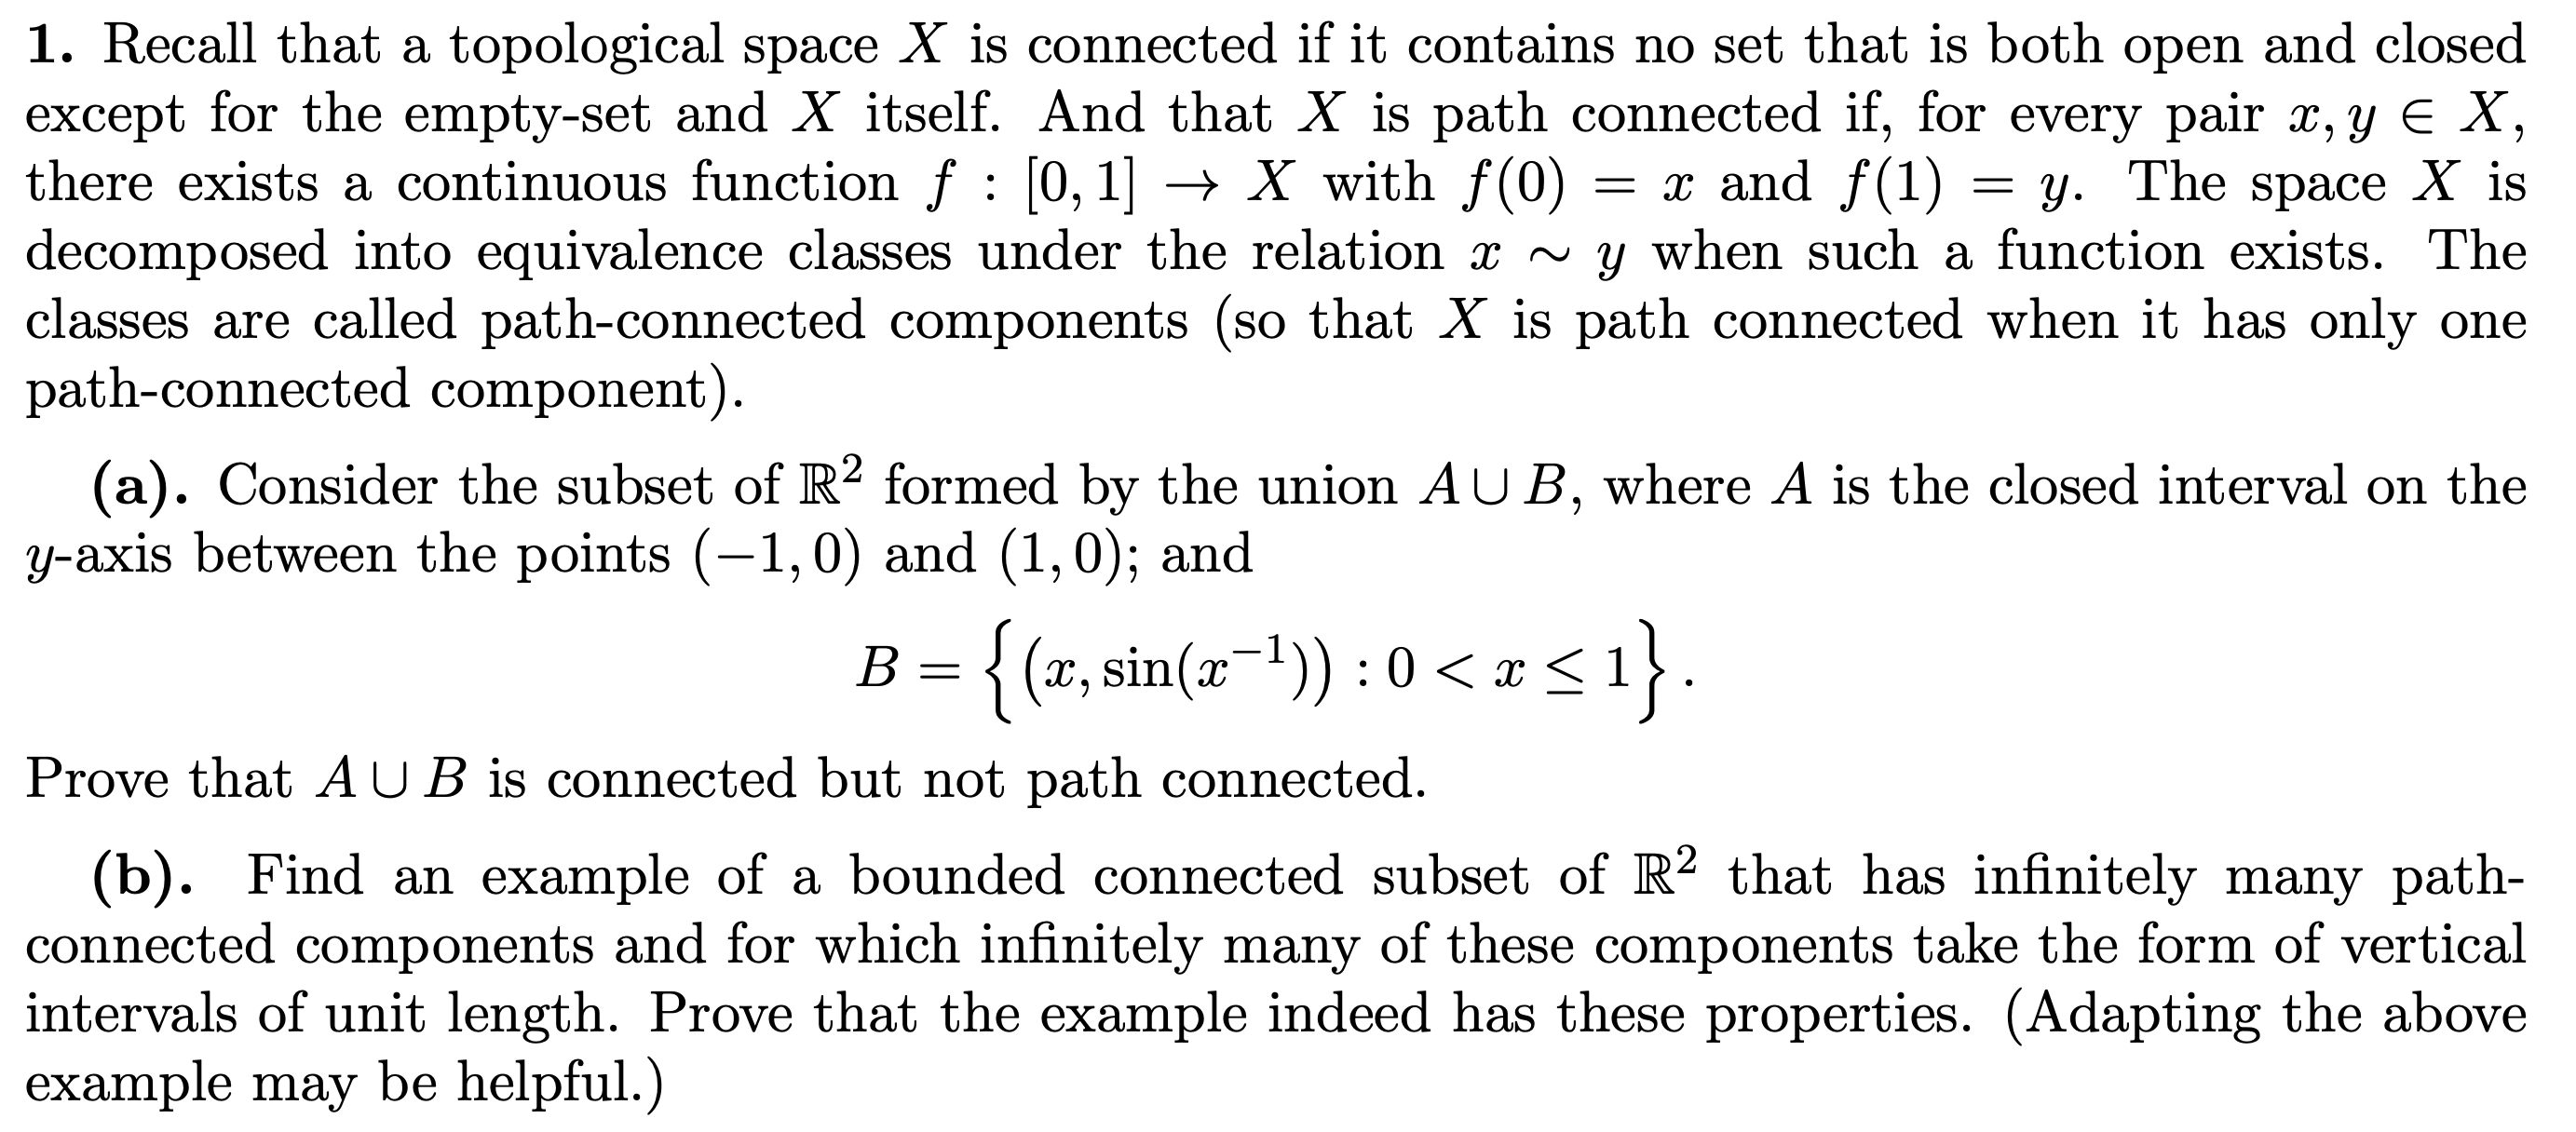
\includegraphics[width=400pt]{img/analysis--berkeley-202a-hw13-26dd.png}
\end{mdframed}

Recall that a set is closed by definition if its complement is open.

Therefore a set is both open and closed (clopen) iff it is open and its complement is open.

Therefore (no non-trivial clopen sets) $\iff$ (cannot be partitioned into two disjoint open sets)

\begin{claim*}
  $A \union B$ is connected.
\end{claim*}

\begin{proof}
  We must show that $A \union B$ cannot be written as the union of two disjoint non-empty open sets.

  Suppose for a contradiction that $U$ and $V$ are disjoint open sets such that $U \union V = A \cup B$.
  Let $z \in B$ and without loss of generality suppose that $z \in V$. Then $B \subseteq V$ (since $B$ is
  connected). Note that the open ball at $(0, 0)$ contains a point of $B$. But $U$ and $V$ are disjoint,
  therefore $(0, 0) \in V$. But $(0, 0) \in A$ and $A$ is connected, so $A \subseteq V$.
  Therefore $A \union B = V$. But this is a contradiction since $U$ and $V$ are disjoint and non-empty.
  Therefore $A \union B$ are connected.
\end{proof}


\begin{claim*}
  $A \union B$ is not path-connected.
\end{claim*}

\begin{proof}
  Suppose for a contradiction that there exists a continuous function $f: [0, 1] \to A \union B$ such
  that $f(0) = (0, 0)$ and $f(1) = (0, 1)$.

  Suppose for a contradiction that there exists a continuous function $f: [0, 1] \to A \union B$ such
  that $f(0) = (0, 1)$ and $f(1) = (0, 0)$.

  Write $f = (f_x, f_y)$ where $f_x: [0, 1] \to [0, 1]$ and $f_y: [0, 1] \to [-1, 1]$ give the coordinates of $f$.

  Let $\eps > 0$ and let $(t_n)_{n=1}^\infty$ be an increasing sequence with $0 < t_n < 1$ and $t_n \to 1$.
  Then $f_y(t_n) \to 0$ since $f$ is continuous. Let $N$ be such that $f_y(t_n) < \eps$ for all $n \geq N$. But
  this is a contradiction since $f_y (t_n))$ is oscillating between $-1$ and $1$ but $\eps$ is arbitrary.
  Therefore no such continuous function $f$ exists.
\end{proof}


\newpage
\begin{mdframed}
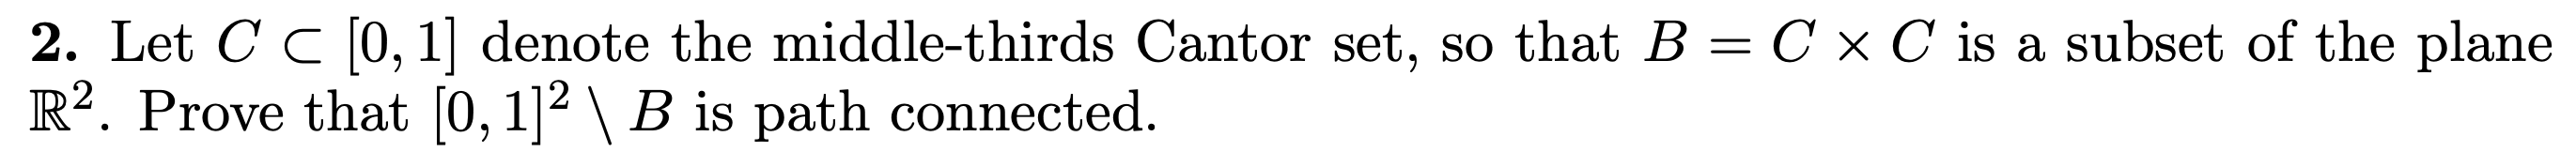
\includegraphics[width=400pt]{img/analysis--berkeley-202a-hw13-e2f7.png}
\end{mdframed}

\newpage
\begin{mdframed}

\includegraphics[width=400pt]{img/analysis--berkeley-202a-hw13-983a.png}
\end{mdframed}

\begin{proof}
  This is theorem 20.30 of Bass; the proof is given there. The theorem states that if $X$ is compact Hausdorff
  then $X$ is normal, and the conditions asked for here are part of the definition of normal.\\
  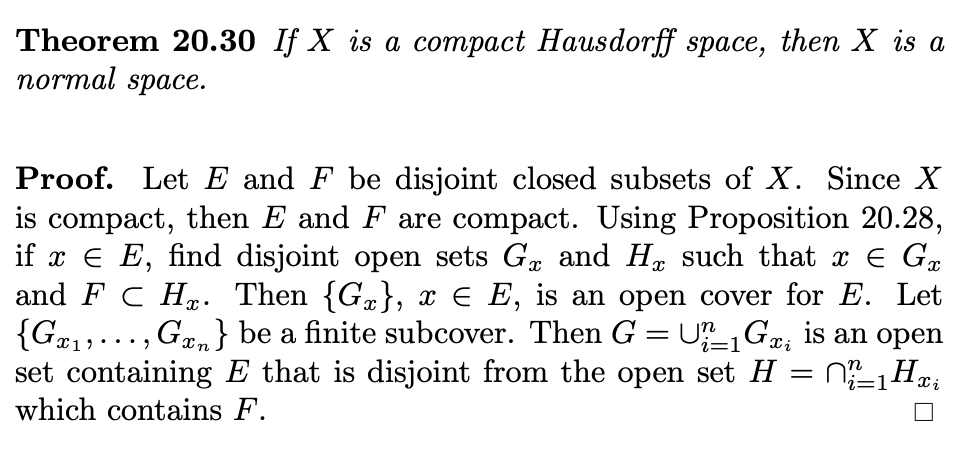
\includegraphics[width=400pt]{img/analysis--berkeley-202a-hw13-7531.png}
\end{proof}


\newpage
\begin{mdframed}
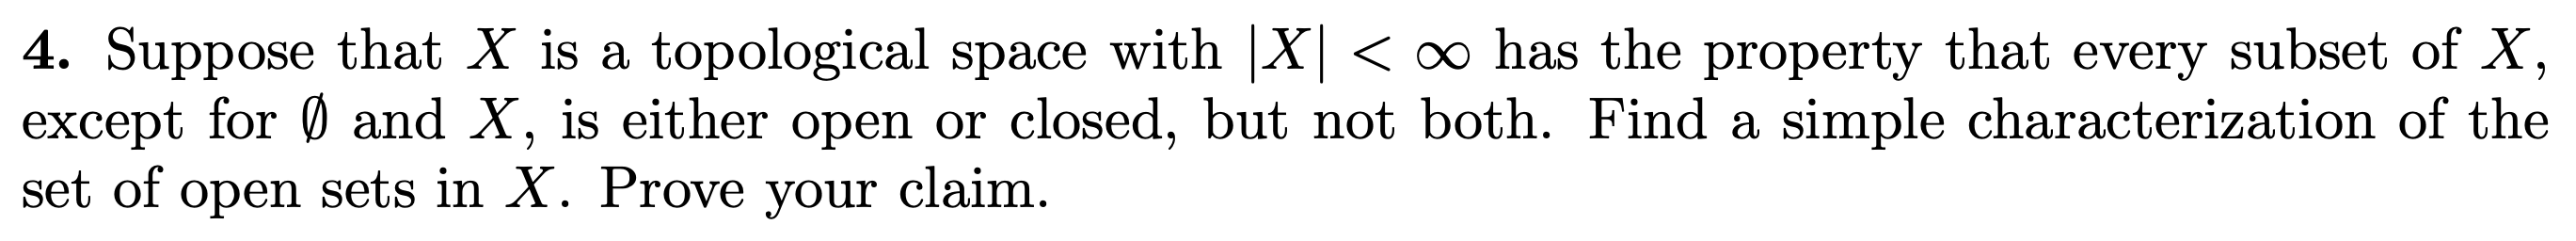
\includegraphics[width=400pt]{img/analysis--berkeley-202a-hw13-9356.png}
\end{mdframed}

First, let's examine some small finite sets and the possible topologies that meet the specified condition. The
following table excludes topologies that differ only by a relabeling of the elements in the underlying set.

\begin{tabular}{l|l|l}
  set&non-trivial&non-trivial\\
     &open subsets&closed subsets \\
  \hline
  $\{\}$             &                                                                                                 & \\
  \hline
  $\{1\}$            &                                                                                                 & \\
  \hline
  $\{1, 2\}$         & $\{1\}$                                                                                         & $\{2\}$\\
  \hline
  $\{1, 2, 3\}$      & $\{1\}$                                                                                         & $\{2, 3\}$ \\
  $\{1, 2, 3\}$      & $\{1\}, \{2\}, \{1, 2\}$                                                                        & $\{2, 3\}, \{1, 3\}, \{3\}$ \\
  $\{1, 2, 3\}$      & $\{1\}, \{1, 2\}$                                                                               & $\{2, 3\}, \{3\}$ \\
  $\{1, 2, 3\}$      & \sout{$\{1\}, \{2, 3\}$}                                                                        & \sout{$\{2, 3\}, \{1\}$} \\
  $\{1, 2, 3\}$      & $\{1, 2\}$                                                                                      & $\{3\}$ \\
  $\{1, 2, 3\}$      & \sout{$\{1\}, \{2\}, \{1, 2\}, \{3\}, \{1, 3\}, \{2, 3\}$}                                      & \sout{$\{2, 3\}, \{1, 3\}, \{3\}, \{1, 2\}, \{2\}, \{1\}$} \\
  $\{1, 2, 3\}$      & \sout{$\{1\}, \{2\}, \{1, 2\}, \{1, 3\}$}                                                       & \sout{$\{2, 3\}, \{1, 3\}, \{3\}, \{2\}$} \\
  \hline
  $\{1, 2, 3, 4\}$   & $\{1\}$                                                                                         & $\{2, 3, 4\}$ \\
  $\{1, 2, 3, 4\}$   & $\{1\}, \{2\}, \{1, 2\}$                                                                        & $\{2, 3, 4\}, \{1, 3, 4\}, \{3, 4\}$ \\
  $\{1, 2, 3, 4\}$   & $\{1\}, \{1, 2\}$                                                                               & $\{2, 3, 4\}, \{3, 4\}$ \\
  $\{1, 2, 3, 4\}$   & $\{1\}, \{2, 3\}, \{1, 2, 3\}$                                                                  & $\{2, 3, 4\}, \{1, 4\}, \{4\}$ \\
  $\{1, 2, 3, 4\}$   & $\{1\}, \{1, 2, 3\}$                                                                            & $\{2, 3, 4\}, \{4\}$ \\
  $\{1, 2, 3, 4\}$   & \sout{$\{1\}, \{2, 3, 4\}$}                                                                     & \sout{$\{2, 3, 4\}, \{1\}$} \\
  $\{1, 2, 3, 4\}$   & $\{1, 2\}$                                                                                      & $\{3, 4\}$ \\
  $\{1, 2, 3, 4\}$   & \sout{$\{1, 2\}, \{3, 4\}$}                                                                     & \sout{$\{3, 4\}, \{1, 2\}$} \\
  $\{1, 2, 3, 4\}$   & $\{1\}, \{2\}, \{1, 2\}, \{3\}, \{1, 3\}, \{2, 3\}, \{1, 2, 3\}$                                & $\{2, 3, 4\}, \{1, 3, 4\}, \{3, 4\}, \{1, 2, 4\}, \{2, 4\}, \{1, 4\}, \{4\}$ \\
  $\{1, 2, 3, 4\}$   & \sout{$\{1\}, \{2\}, \{1, 2\}, \{3\}, \{1, 3\}, \{2, 3\}, \{1, 2, 3\}$},                        & \sout{$\{2, 3, 4\}, \{1, 3, 4\}, \{3, 4\}, \{1, 2, 4\}, \{2, 4\}, \{1, 4\}, \{4\}$}, \\
                     & ~~~~\sout{$\{4\}, \{1, 4\}, \{2, 4\}, \{1, 2, 4\}, \{3, 4\}, \{1, 3, 4\}, \{2, 3, 4\}$}         & ~~~~\sout{$\{1, 2, 3\}, \{2, 3\}, \{1, 3\}, \{3\}, \{1, 2\}, \{2\}, \{1\}$} \\
\end{tabular}

\newpage
\begin{mdframed}
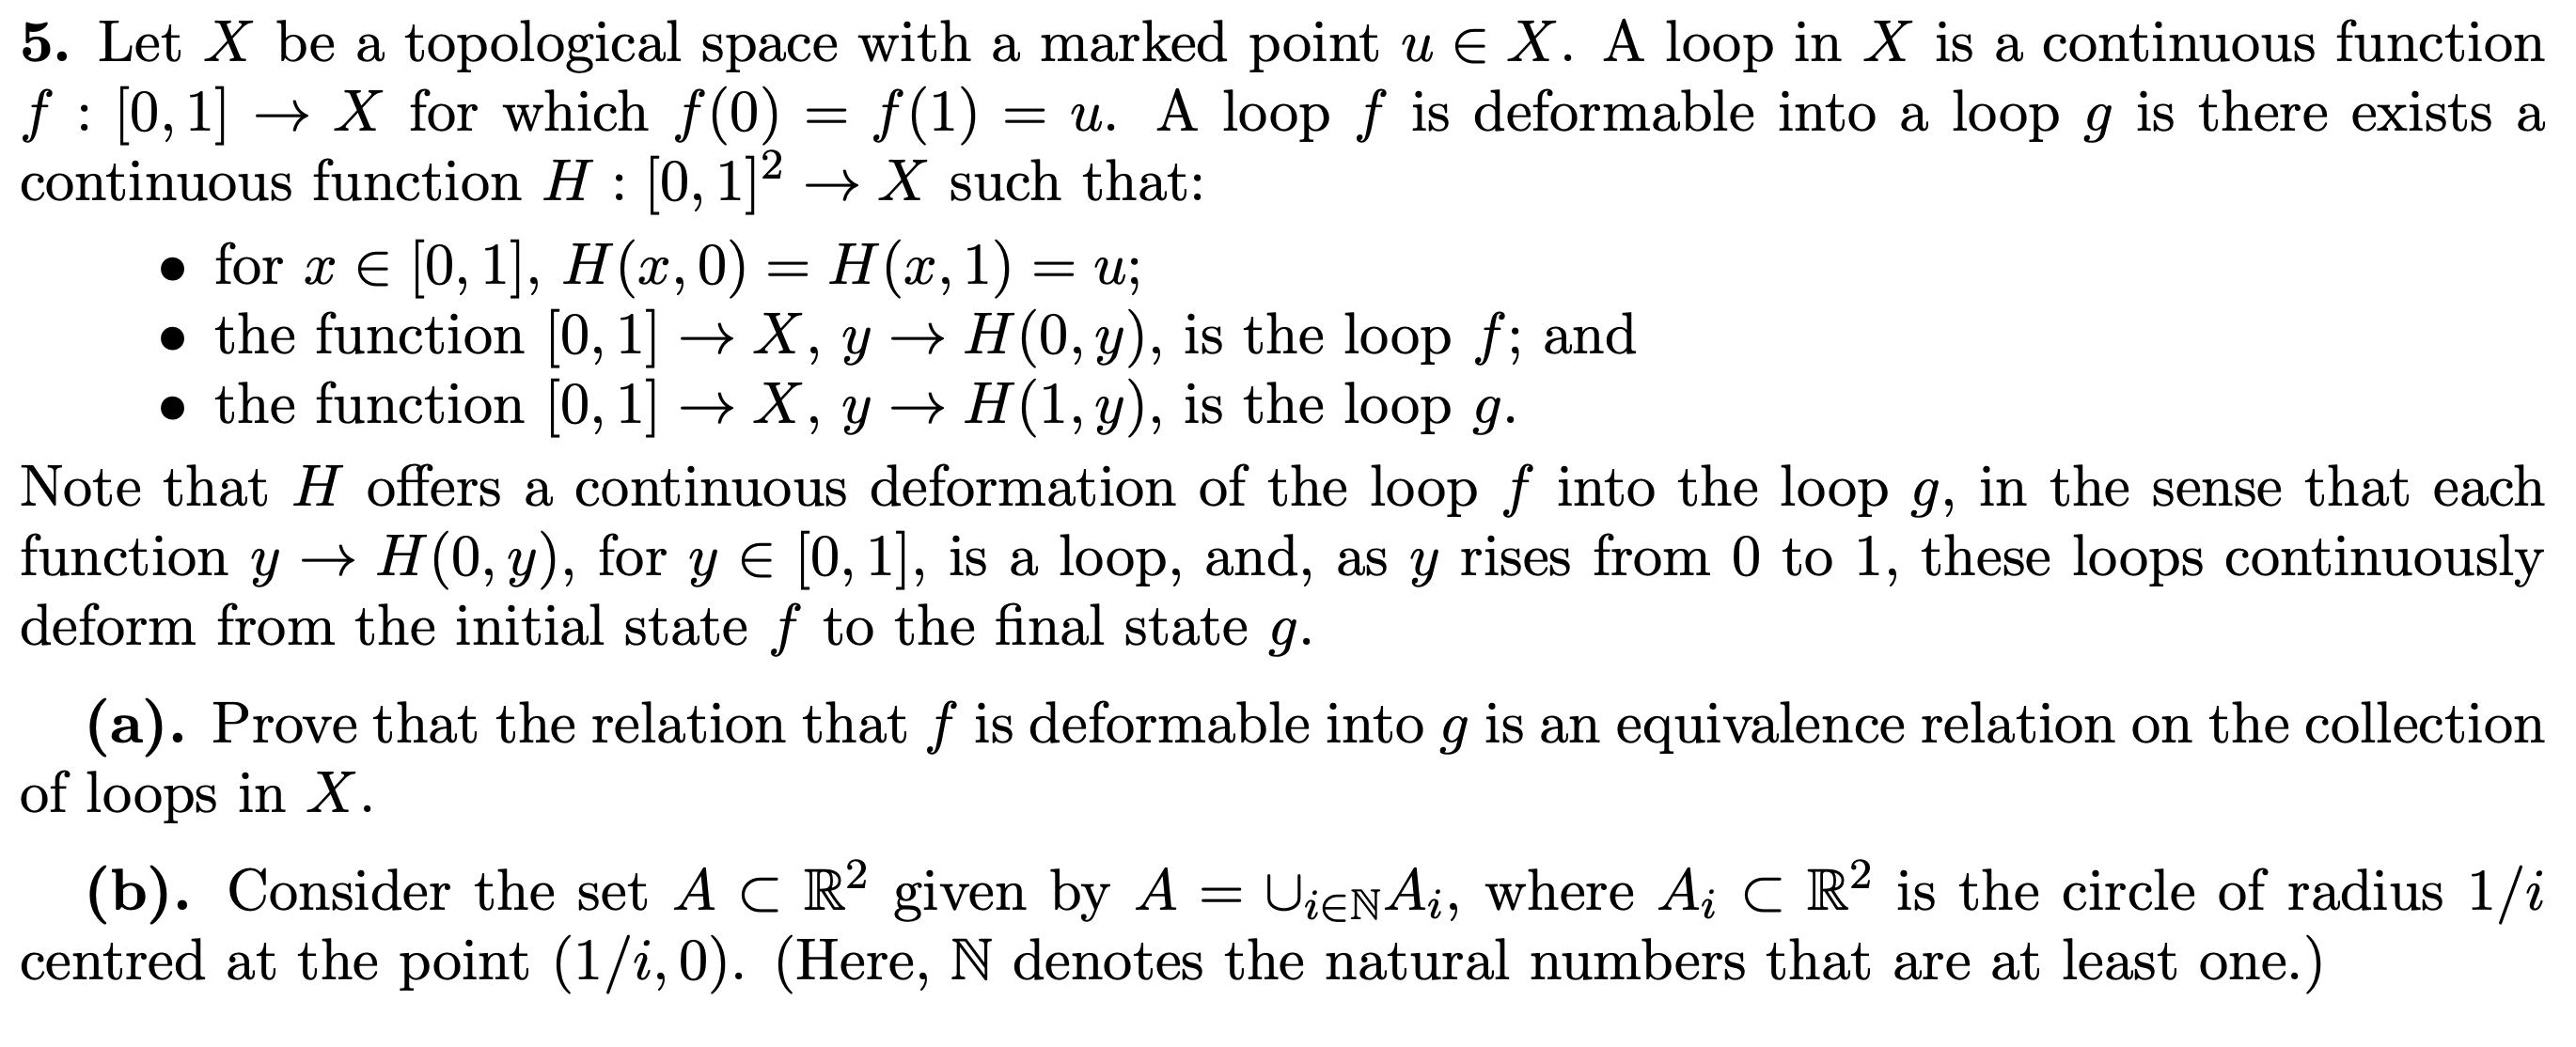
\includegraphics[width=400pt]{img/analysis--berkeley-202a-hw13-aa83.png}\\

\includegraphics[width=400pt]{img/analysis--berkeley-202a-hw13-f49f.png}
\end{mdframed}
